\documentclass[12pt,oneside]{report}
\usepackage{setspace}
\usepackage{amsmath}
\usepackage[pdftex]{graphicx}
\usepackage{suthesis-2e}
\usepackage{hyperref}
\usepackage{multirow}
\usepackage{todonotes}
\usepackage{tikz}
\usepackage{upgreek}
\usepackage{gantt}
\usepackage{listings}
\usepackage{booktabs, colortbl, tabularx}
\definecolor{gainsboro}{rgb}{0.96,0.94,0.93}
\usepackage{xcolor}
%\lstset{language=C,
%           basicstyle=\ttfamily\tiny,
%           backgroundcolor=\color{black!5}, % set backgroundcolor
%           keywordstyle=\color{blue}\ttfamily,
%           stringstyle=\color{red}\ttfamily,
%           commentstyle=\color{green}\ttfamily,
%          breaklines=true
%          }
\usepackage{calc}
\usepackage{array}
\usepackage{rotating}
\usepackage{url}
\usepackage{pgf,tikz}
\usetikzlibrary{snakes,arrows,shapes}
\usepackage{adjustbox}
\usepackage{dot2texi}
\usepackage[normal]{subfigure}
\usepackage{multirow}
\usepackage{todonotes}
\usepackage{tikz}
\usepackage{xcolor}
\usepackage{pgfplots, pgfplotstable}
\usepackage{amsmath}
\usepackage{pgf,tikz}
\usetikzlibrary{snakes,arrows,shapes}
\usepackage{amsmath}
\usepackage{mdwlist}
\usepackage{xcolor}
\usepackage{adjustbox}
\usepackage{dot2texi}



\usepackage{pgfplots, pgfplotstable}
\usepackage{amsmath}
\makeatletter
\newif\if@restonecol
\makeatother
\let\algorithm\relax
\let\endalgorithm\relax
\usepackage[ruled]{algorithm2e}
\usepackage{multirow}
\usepackage[center]{caption}
\usepackage{xcolor}
\usepackage{tikz}
\usepackage{calc}
\def\checkmark{\tikz\fill[scale=0.4](0,.35) -- (.25,0) -- (1,.7) -- (.25,.15) -- cycle;} 
\def\scalecheck{\resizebox{\widthof{\checkmark}*\ratio{\widthof{x}}{\widthof{\normalsize x}}}{!}{\checkmark}}
\usetikzlibrary{arrows,backgrounds}
\usetikzlibrary{arrows,automata,calc,shapes,positioning,shadows,trees}

\pgfplotsset{compat=newest}


\tikzset{
  basic/.style  = {draw, text width=2cm, font=\sffamily, rectangle},
  root/.style   = {basic, rounded corners=2pt, thin, align=center,
                   fill=white!90},
  level 2/.style = {basic, rounded corners=6pt, thin,align=center, fill=white!90,
                   text width=8em},
  level 3/.style = {basic, thin, align=left, fill=white!90, text width=6.5em}
}


%\usepackage{acro}
\usepackage{acronym}
\usepackage{color}
\definecolor{lightgray}{rgb}{0.95, 0.95, 0.95}
\definecolor{darkgray}{rgb}{0.4, 0.4, 0.4}
\definecolor{purple}{rgb}{0.65, 0.12, 0.82}
\definecolor{ocherCode}{rgb}{1, 0.5, 0} % #FF7F00 -> rgb(239, 169, 0)
\definecolor{blueCode}{rgb}{0, 0, 0.93} % #0000EE -> rgb(0, 0, 238)
\definecolor{greenCode}{rgb}{0, 0.6, 0} % #009900 -> rgb(0, 153, 0) 
\usepackage{upquote}
\usepackage{listings}
\makeatletter
%\lstdefinelanguage{HTML5}{
%	sensitive=true,
%	keywords={%
%		% JavaScript
%		typeof, new, true, false, catch, function, return, null, catch, switch, var, if, in, while, do, else, case, break,
%		% HTML
%		html, title, meta, style, head, body, script, canvas,
%		% CSS
%		border:, transform:, -moz-transform:, transition-duration:, transition-property:,
%		transition-timing-function:
%	},
%	% http://texblog.org/tag/otherkeywords/
%	otherkeywords={<, >, \/},   
%	ndkeywords={class, export, boolean, throw, implements, import, this},   
%	comment=[l]{//},
%	% morecomment=[s][keywordstyle]{<}{>},  
%	morecomment=[s]{/*}{*/},
%	morecomment=[s]{<!}{>},
%	morestring=[b]',
%	morestring=[b]",    
%	alsoletter={-},
%	alsodigit={:}
%}



\usepackage{booktabs}
\usepackage{array}
\usepackage{caption}
%\usepackage{subcaption}
\usepackage{multirow}
\usepackage{rotating}
\usepackage{url}
\usepackage{tikz}
%\usetikzlibrary{dsp,chains}
\usepackage{pgf,tikz}
\usetikzlibrary{calc,arrows}
\usepackage{amsmath}
%\usepackage{titlesec}
%\usepackage{ulem}
%\usepackage{subfigure}
%\usepackage{subcaption}
\setcounter{secnumdepth}{4}
\setcounter{tocdepth}{4}
%\setcounter{secnumdepth}{4}
%\setcounter{tocdepth}{4}
\renewcommand{\topfraction}{0.9}	% max fraction of floats at top
\renewcommand{\bottomfraction}{0.8}	% max fraction of floats at bottom
%Parameters for TEXT pages (not float pages):
\setcounter{topnumber}{2}
\setcounter{bottomnumber}{2}
\setcounter{totalnumber}{4}     % 2 may work better
\setcounter{dbltopnumber}{2}    % for 2-column pages
\renewcommand{\dbltopfraction}{0.9}	% fit big float above 2-col. text
\renewcommand{\textfraction}{0.07}	% allow minimal text w. figs
%Parameters for FLOAT pages (not text pages):
\renewcommand{\floatpagefraction}{0.7}	% require fuller float pages
%N.B.: floatpagefraction MUST be less than topfraction !!
\renewcommand{\dblfloatpagefraction}{0.7}	% require fuller float pages
%remember to use [htp] or [htpb] for placement

\newenvironment{packed_enum}{
\begin{enumerate}
  \setlength{\itemsep}{1pt}
  \setlength{\parskip}{0pt}
  \setlength{\parsep}{0pt}
}{\end{enumerate}}

\graphicspath{{figures/}}
\begin{document}



\begin{titlepage}
\begin{center}
{\LARGE {NANYANG TECHNOLOGICAL UNIVERSITY}}
\begin{figure}[!t]
\centering

\includegraphics[width= 8 cm]{figures/ntu_logo.pdf}
\end{figure} 
\vspace*{0.7in}
{\large OPENCL SUPPORT FOR ACCELERATORS ON ZYNQ USING PORTABLE COMPUTING LANGUAGE (pocl)}
\par
\vspace{0.4 in}
{\large by\\}
\vspace{0.2 in}
{\large SETHUPANDI ABISHEK

(G1601372F)}
\vspace{0.1 in}
\par
\vfill
A Dissertation Submitted in partial fulfillment of \\ the requirements for the degree of \\ Master of Science in Embedded Systems
\par
\vspace{0.4in}
Supervised by\\
%\par
\vspace{0.1in}
{\large Assoc. Prof. Douglas L. Maskell \\}
\par
\vspace{0.15in}
July 2017
\end{center}
\end{titlepage}
%\onehalfspacing
\pagenumbering{roman}
\tableofcontents
\listoffigures
\addcontentsline{toc}{chapter}{List of Figures}	
\listoftables
\addcontentsline{toc}{chapter}{List of Tables}

%\thispagestyle{plain}
%\newpage
%\thispagestyle{plain}
%\printacronyms[include-classes=abbrev,name=Abbreviations]
%\thispagestyle{plain}

\newpage
\chapter*{Abbreviations}
\addcontentsline{toc}{chapter}{Abbreviations}
\begin{acronym}[MPC]\itemsep0pt % Give the longest label here so that the list is nicely aligned
\acro{API}{Application Programming Interface}
\acro{BRAM}{Block Random Access Memory}
\acro{CLB}{Configurable Logic Block}
\acro{DMA}{Direct Memory Access}
\acro{DVFS}{Dynamic Voltage and Frequency Scaling}
\acro{FIFO}{First In First Out}
\acro{FPGA}{Field Programmable Gate Arrays}
\acro{HSA}{Heterogeneous System Architecture}
\acro{MPPA}{Massively Parallel Processor Array}
\acro{OPENCL}{Open Computing Language}
\acro{POCL}{Portable Computing Language}
\acro{PCI}{Peripheral Component Interconnect}
\acro{PAPI}{Performance Application Programming Interface}
\acro{SPMD}{Single Program Multiple Data}
\acro{SIMT}{Single Instruction Multiple Thread}
\acro{TLP}{Thread Level Parallelism}
\acro{TTA}{Transport Triggered Architecture}
\acro{VLIW}{Very Long Instruction Word}
\end{acronym}

\begin{abstract}
 
Heterogeneous System Architecture has become a new era for computing in an optimal way and Reconfigurable Platforms are promising for better acceleration in HSA Platforms. OpenCL Standard are introduced for writing parallel programs to heterogeneous systems. This framework simplifies the usage of accelerators for programmers in software. Portable Computing Language software is used for OpenCL implementation. The modularized form of POCL's software architecture supports the addition of new device for OpenCL Implementation. In thesis work, we integrate OpenCL Drivers for Zynq platform using xillybus in POCL. Xillybus project provides FPGA IP core design with efficient DMA based solution for data transport between Linux or Windows to FPGA device. The new device called 'xillybus' is available as OpenCL device for Programmable Logic. While, Processing System is supported using 'pthread', which is available as a default device in POCL. The POCL package is installed on Xillinux distribution for Zedboard and steps to integrate xillybus drivers is also discussed. An OpenCL host application, which has a kernel function to perform vector addition, is developed that can execute on both CPU and FPGA devices. POCL's OpenCL data transfer APIs are profiled using PAPI library, where read and write APIs of xillybus device transfers faster than the pthread device when the number of samples is increased. An introduction to OpenCL runtime using POCL is discussed. This work enables using accelerator with xillybus project that can support OpenCL Standard with OpenCL Runtime compiler integration on Zynq Platform.
  
\end{abstract}

\chapter*{Acknowledgment} 
\label{ch0_Acknowledgement}
I would like to express my deep and sincere gratitude to Assoc. Prof. Douglas Leslie Maskell, for his constant and continuous support, encouragement and guidance. I would also like to acknowledge the crucial role of mentor Dr. Abhishek Kumar Jain, for his continuous support, effective suggestions and professional guidance in the entire phase of my dissertation. I sincerely thank him for arranging weekly meeting which were helpful in discussing the project to find the right path to proceed. I would also like to thank my friends and classmates for helping me with technical issues regarding my practical work. My heartfelt appreciation goes to my beloved parents for their support and love throughout my studies at the University. Finally, I would like to thank School of Computer Engineering, Nanyang Technological University, Singapore for their support.

\pagenumbering{arabic}

\chapter{Introduction}
\label{ch1_introduction}

Modern computing environment are becoming heterogeneity with multi-core microprocessors, Central Processing Units(CPU), Graphics Processing Unit(GPU), Digital Signal Processors and Reconfigurable Hardware (FPGAs). In earlier decades, the technology trend scales the performance with increase in transistor density and has more logic functionality in a chip. Since around 2005-2007, Dennard Scaling has broken down due to increase in static power at higher clock frequencies, the Multiple processor cores era begins with the similar cores operating at different frequencies. Multicore processing technology exploits thread level parallelism (TLP) by allowing the programmer to dynamically adjust the voltage and frequency with respect to performance. This technique is called as Dynamic voltage and frequency scaling (DVFS). It is also possible to switch off some part of silicon in the chip, called ‘dark silicon’ so that the heat dissipation can be avoided \cite{1}.

Due to different workload behavior of the applications, the throughput depends on the computation and communication efficiency of the underlying architecture. For example, Control intensive applications can execute faster on CPUs and data intensive applications can execute efficiently in vector architecture. Thus, the modern computing method shifts to Heterogeneous System Architecture(HSA). HSA supports the programmer to select better architecture to execute tasks in an optimal way. Co-processors and accelerators are used extensively for computationally intensive applications. However, the key problem is to communicate the data from the host to accelerators and to manage the threads. Hence, a heterogeneous programming framework called Open Computing Language (OpenCL) standard is maintained for writing parallel codes. OpenCL framework supports multicore platforms, digital signal processors, GPUs and FPGA.

\section{Motivation}
The open source community has developed many software frameworks for OpenCL implementation. Portable Computing Language (POCL) aims to become an MIT licensed OpenCL standard. POCL can be easily portable for CPU, heterogeneous GPUs and accelerators. In this thesis work, we explore POCL software framework to add a new device with OpenCL driver integration.

\section{Contribution}
The main contribution of this thesis is basic OpenCL implementation for Field Programmable Gate Array (FPGA) and Central Processing Unit (CPUs). The contributions are summarized as follows:
\begin{itemize} 
	\item An introduction for adding a FPGA device to POCL software framework in device layer implementation.
	\item Setting up OpenCL standard in Ubuntu distribution on Zynq heterogeneous platform.
	\item Integration of OpenCL drivers in device layer of POCL using xillybus Linux driver.
	\item Testing of OpenCL APIs for data transfer from host to FPGA device.
\end{itemize}

\section{Organization}
The thesis is organized as follows. Chapter 2 discusses background and previous work on implementation of OpenCL standard. In Chapter 3 we describe the concepts of OpenCL Implementation using POCL and its relation to POCL software framework. Chapter 4 discusses the advantage of xillybus project that can be used as an OpenCL driver. Chapter 5, we implement OpenCL library on Zed board and testing data transfer OpenCL APIs. Finally, Chapter 6 concludes the thesis with future work.
\chapter{Background}
\label{ch2_background}

\section{FPGA for Heterogeneous System}
The heterogeneous computing platform combines the traditional CPUs and additional compute architectures to accelerate computationally intensive tasks \cite{2}. Some of the examples are GPUs, MPPAs, Floating point units and cryptographic processors. This promises a new way for improved efficiency and energy efficient systems. Accelerating tasks on MPPAs achieves better energy efficient solutions compared to GPUs and CPUs \cite{3}\cite{4}\cite{5}\cite{6}. The application specific design methodology provides another preferred approach to increase efficiency in area, power and speed. But increased time to market and associativity to higher costs hinders the ASIC design deployment.

FPGAs are the most preferred choice for rapid-prototyping the application specific accelerators in heterogeneous system architecture. It also provides flexibility to modify the hosted accelerator even after deployment \cite{7}\cite{8}\cite{9}. The new era of FPGA consists of Configurable Logic blocks (CLBs) connected by I/Os with the additional hard blocks called macros such as DSP blocks and reconfigurable embedded memories like BRAMs. The main concern in reconfigurable architecture is data transfer bandwidth and to use the hardware resources efficiently for the accelerator. Vendor specific hard processors are proposed \cite{10} to provide high bandwidth transfer. With hardware-software partitioning for an application, the hardware tasks are mapped to FPGA fabric using Hardware Description Languages(HDL) like Verilog and VHDL. For rapid design space exploration and to increase marginal performance in area and cost, the next preferred design method must be raising the level of programming abstraction. For example, Vivado HLS, a commercial tool from Xilinx, converts the C algorithmic implementation to RTL code.  

\section{Xilinx Zynq Zedboard}
Xilinx gave their new series of All-Programmable System on Chip (SoC) called Zynq which is a flexible and convincing platform for varied applications. It has a combination of ARM Cortex-A9 processor with FPGA, where these partitions are called as Processing System (PS) and Programmable Logic (PL) parts. Processing system can run a complete Linux Operating System and the programmable logic part can be configured with desired design. The Zynq architecture has a high bandwidth, low latency interfaces between PS and PL. Thus, Zynq platform enables the main processor to control the programmable hardware, which runs high intensive compute applications. Based on Zynq-7000 All-Programmable System on Chip, Xilinx has released a development and evaluation board called Zynq Zedboard. Zedboard consist of Zynq Z7020-clg484 of speed grade -1(MHz) package, which has ARM Cortex-A9 as an application processor for Processing System and reconfigurable fabric. The Processing System has 512MB DDR RAM, hard DMA Controller and double precision floating point unit with common peripherals and memory interfaces. Block diagram of PS is shown in Figure \ref{fig:1}\cite{11}. The main components of the PS are as below

\begin{itemize}\itemsep0em 
	\item Based on ARMv7 ISA, run-time configurable two ARM Cortex-A9 multicore processors.
	\item Neon 128b SIMD coprocessor and VFPv3 per processor.
	\item 32KB instruction and L1 data caches per processor.
	\item 512KB L2 cache that is shared between the processors.
	\item Snoop Control Unit (SCU) and the ACP for cache coherent accesses.
	\item On-Chip Memory (OCM) with capacity of 256KB.
	\item DDR controller comprising of AXI memory port interface, digital PHY and transaction scheduler.
	\item DMA controller with four channels for PS and PL.
\end{itemize}
\begin{figure}[h]
    \centering
    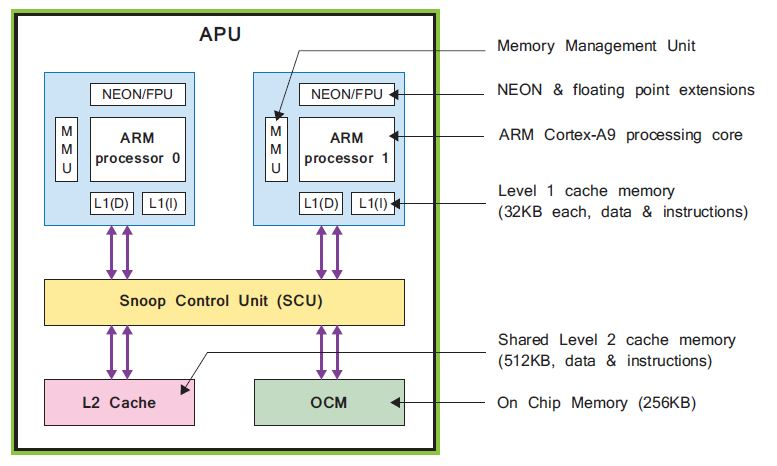
\includegraphics[width=0.90\textwidth]{Processing_system}
    \caption{Block Diagram of Processing System}
    \label{fig:1}
\end{figure}

The programmable logic part is made up of Artix 7 FPGA fabric. The PL can be configured partially or fully with the configuration data as a bitstream. The PL power can be managed for real time applications. The configurations of PL are listed below \cite{23}.

\begin{itemize}\itemsep0em 
	\item 36KB block RAM with capability of dual port.
	\item DSP48E1 Slice with optional pipelining, ALU and dedicated buses for cascading useful for Digital signal processing.
	\item Low jitter clock distribution and low skew.
	\item High performance I/O that can be configured.
	\item Dual Analog-to-Digital Converter (ADC) blocks with 12-bit and 1 MSPS rate.
\end{itemize}

The Zynq platform uses multiple AXI channels for communication between PS and PL. There are three types of AXI interfaces shown below.
\begin{itemize}\itemsep0em 
	\item Two 32-bit, AXI master and slave general purpose ports -- AXI\_GP.
	\item Four 32/64-bit, AXI slave high performance ports -- AXI\_HP.
	\item One 64-bit configurable, AXI slave Accelerator Coherency Port -- AXI\_ACP.
\end{itemize}

\section{OpenCL}
Open Computing Language (OpenCL) is a framework for heterogeneous programming, managed by non-profit consortium Khronos group. OpenCL APIs are restricted version of C99 language that can be used for developing parallel code for various computing devices like CPUs, GPUs, Accelerated Processing Unit. OpenCL C Code is called as program, comprises of collection of functions called kernels. Kernels are the basic part of the OpenCL Program that executes on the device. OpenCL guides the programmer to develop OpenCL targeted parallel program. It offers both Host management layer and Device layer. Host management layer or a host program is executed by the user and manages the number of devices in the system for kernel execution. While, Device layer is designed for mapping the parallel code to the selected device. OpenCL specification is categorized into four basic models. They are Platform model, Execution model, Memory model and Programming model.

\subsection{Platform Model}
The single host directs execution on one or more devices as shown in the figure \ref{fig:2}. Platforms are vendor specific implementation of OpenCL APIs. It is the abstract way of representing the devices in a heterogeneous system. Vendor maps the abstract architecture to physical hardware. In simple ways, if programmer chooses vendor A’s platform, he cannot communicate vendor B’s GPU in the same system.  The platform model defines the compute device as an array of compute units like some of the GPU model and each compute unit is further divided into processing elements (PE). The OpenCL API function clGetPlatformIDs() discovers the available number of platforms for a given system. The compute devices can be identified by clGetDeviceIDs() with following device types like CPU, GPU or Accelerator. The device\_type argument is used to limit the required devices for selection by a programmer.
\begin{figure}[h]
    \centering
    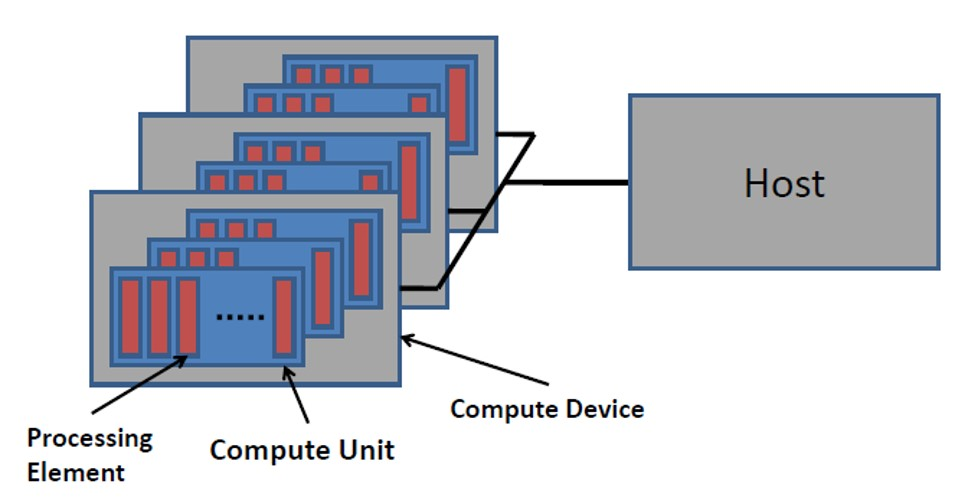
\includegraphics[width=0.80\textwidth]{Platform_Model}
    \caption{Platform Model}
    \label{fig:2}
\end{figure}

\subsection{Execution Model}
A context is created for managing the execution of OpenCL Commands, which includes data movement and kernel execution. A Kernel program is available as a source in ISO C99 standard with several extensions. Host program builds the kernel program to map accordingly to the device using clBuildProgram() API. A kernel instance is created for each index available, based on the index space for a device. Each kernel instance is called work item. Work item are the basic unit for concurrent execution. To facilitate the scalability, the work items in N – dimensional range is divided into equal work group sizes. It can be specified as one, two or three-dimensional vectors. Work group size is fixed to a specific group size for efficient hardware implementation. Work items are executed with the function call to clEnqueueNDRangeKernel().
\begin{figure}[h]
    \centering
    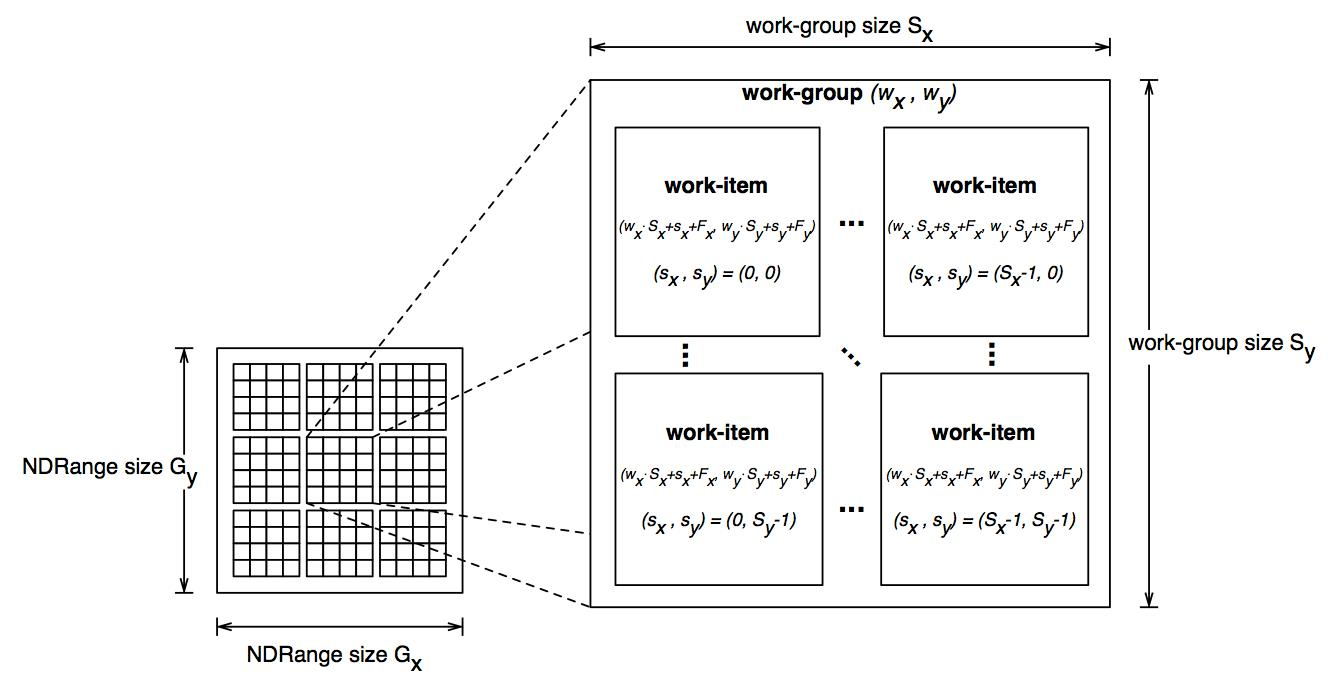
\includegraphics[width=1\textwidth]{execution_model}
    \caption{An Example of 2-dimensional index space}
    \label{fig:3}
\end{figure}
For Example, A hardware with two-dimensional index space has Gx by Gy work items. Figure \ref{fig:3} \cite{12} contains nine work groups with each of size Sx by Sy. Work-groups are assigned with an ID (wx, wy) and work items have local and global ID. Global ID are assigned using global offset called Fx and Fy. 

\subsection{Memory Model}
OpenCL defines an abstract model to map the memory space into hardware. Usually the memory subsystems differ between platforms. For example, CPU has automatic cache system while GPUs do not support. Thus, OpenCL C language provides four address spaces called private, local, global and constant. Programmer uses keywords to associate the memory space for variable. Global memory is visible to all compute units on the device. The initial data transfer from host to device will reside in global memory. Constant memory is accessed simultaneously by all the work items and it is designed for read only. Local memory is shared between work groups and it is unique for each compute device. Whereas Private memory is unique to an individual work items. The memory model of OpenCL is closely related to modern GPUs.

Hence, the platform model defines the host and device. The kernel creation and execution are set up by the hosts using execution model with required space for parallelism. Then data transfers and memory space are managed using memory model. Contexts and kernel are created and mapped using programming model. A typical OpenCL Implementation requires all the above model. The OpenCL runtime and driver will map the memory spaces to the physical hardware.

\section{Related Work}
LE1 \cite{13}, a customized VLIW chip multiprocessor is designed with unified compilation strategy. A LLVM compilation prototype was developed to enable the OpenCL application execution on LE1 CPU. The compilation flow automates the coalescing of work items for better utilization of cores available. LE1 provides super linear performance with certain improvements from compiler optimization.

An Accelerator based on $\uprho$-VEX Processor \cite{14} is implemented on ML605 Platform. The ρ-vex processor is a VLIW processor instantiated on FPGA and it is interfaced to the host system using PCI Express Bus. To abstract the accelerator in software, OpenCL framework has been developed. The communication interface is developed as Linux kernel drivers, which is used as OpenCL Drivers. With the available LLVM backend for ρ-Vex processor, a runtime support can be integrated in OpenCL framework. OpenCL drivers and runtime for accelerator are implemented using POCL’s OpenCL framework. The key features are analyzing execution time with three main contributing factors. They are data transfer throughput, kernel compile time and kernel execution time. The proposed accelerator achieved 1.2 to 0.11 times the performance of modern GPUs.

Texas Instrument’s System on Chip (ARM as host and DSP as device)\cite{15} and DSP device with PCI-E interface supports OpenCL framework. TI’s Kernel compilation flow for OpenCL devices uses LLVM passes from POCL. It also supports both online and offline kernel compilation. With LLVM passes, the kernel functions or work items are transformed into work group functions.

\chapter{OpenCL Implementation using POCL}
\label{ch3_OpenCL_Implementation_using_POCL}

This Chapter discusses OpenCL implementation using Portable Computing Language. It introduces software architecture and modularizing nature of POCL’s kernel compiler. This chapter also covers the device layer modification required for OpenCL Drivers.

\section{POCL}
POCL, Portable Computing Language is an open source implementation of OpenCL standard. It aims to become an MIT licensed standard. The key feature of pocl is to support OpenCL easily for new devices and targets. The latest version of pocl has been implemented for homogeneous CPUs and heterogeneous GPUs like NVIDIA using CUDA backend. Earlier, OpenCL standard Implementations are vendor and platform specific. Kernel function needs to be optimized depending on the underlying hardware. For SPMD style architecture, the program needs to be synchronized with multiple work-items. The main concept is the work groups that executes the work items should not have data dependencies with other work items, which execute in parallel. This requires the programmer a clear understanding of the platform to tune the program through OpenCL Implementation. In addition, to achieve performance portability, there is a necessary to handle each program separately. This becomes a disadvantage when performance portability is considered with manual optimization.

POCL kernel compilation techniques exposes parallelism of multiple work-items in work groups that can be easily optimized in several types of physical hardware. pocl separates the parallel region in kernel functions so that the parallel mapping of multi-WI workgroups is created with required granularity from the available resources. This transformation is modularized as a set of passes using LLVM compiler organization \cite{16}. POCL allows complete OpenCL Implementation for a wide range of architectures (SIMD, VLIW, superscalar) with various degree of parallelism. Kernel Compiler of pocl completely works on LLVM Intermediate representative. LLVM IR supports more kernel languages via Standard Portable Intermediate Representation \cite{17}. The latest version of pocl v0.14 does not fully implement OpenCL standard (both 1.x and 2.x). Still, it can be considered efficient because of modularized kernel compiler. The pocl test suites run most of the test cases and benchmarks like ViennaCL, Rodinia, Parboil and Luxmark v2.0. POCL also extends OpenCL implementation for Android.

POCL has different OpenCL Implementation under the name of pthread, basic, ttasim, hsa and cuda. 'pthread' implements OpenCL Standard for CPU that uses POSIX library to execute work items from kernel function. 'basic' is the example device implementation for CPU which can be used for implementing POSIX compliant operating system. 'ttasim' simulates the implementation for Transport-Triggered Architecture based accelerator using TCE’s (TTA-based Co-design Environment) library. 'hsa' is an experimenting implementation for AMD Kaveri or Carrizo APUs. POCL supports NVIDIA GPUs under the name of 'cuda' as it uses the backend of CUDA driver, that provides open source alternative to NVIDIA OpenCL Implementation. This backend can also be used on ARM based platforms with NVIDIA GPUs such as Jetson TK1 and TX1 development boards.
 
\section{Software Architecture}
The software components of pocl are isolated with device respected features and enhance the re-usability of certain aspects of the implementation. The general implementation is separated into two layers as Figure \ref{fig:4_PM} \cite{18}. They are Host layer implementation and Device layer implementation. First, Host layer has C compiler support. It can be easily portable to host, that has operating system C compiler support.
\begin{figure}[h]
    \centering
    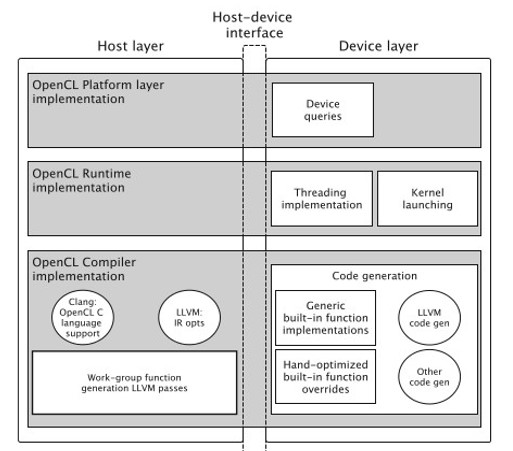
\includegraphics[width=1\textwidth]{soft_arch}
    \caption{POCL Software Framework}
    \label{fig:4_PM}
\end{figure}

Second, Device layer, which is dependent on the physical device, has default devices such as pthread, cuda, basic, ttasim and hsa. It can be found at /lib/CL/devices/ location in pocl. Device layer is responsible for code generation for the target, after performing device dependent optimization. OpenCL framework is C based implementation, which calls the function in device layer through the generic host-device layer. For example, when global memory space is requested from an application for buffer allocation, these queries are processed to device layer through host-device interface.

POCL software architecture offers easy portability for devices. The pthread device layer implementation can be ported for Symmetric Multi-Processing (SMP) systems that support pthread APIs in their operating system. Even ttasim device drivers can communicate and allocate buffers through DMA commands. Another main aspect of POCL is memory management for devices. They provide Bufalloc mechanism for memory allocation so that the buffers are used as a generic memory. The memory region is considered like a memory pools that the chunks of the region are returned based on the availability with every malloc call. 

\section{Platform Layer Implementation}
The platform name is called as Portable Computing Language with platform version as an OpenCL standard version and pocl release version. In OpenCL, we have a platform model to select the available number of devices in the system. Here, the platform layer of pocl queries the available number of devices through host-device layer. However, the device specific queries can be found in the device layer. POCL checks the environmental variable for enabled device. The software components of pocl may contain many OpenCL device implementation but the device can be enabled by environmental variable. This platform query can be found in /lib/CL/devices/device.c. The device specific information like global memory size, local memory varies from device to device. So, it is found under specific device names in basic devices directory, /lib/CL/devices/basic/. In addition, pocl also has device specific extra function calls to compute device. For example, In /lib/CL/devices/cpuinfo.c, it updates the number of parallel compute units or cores available for CPU parallel implementation.

\section{Portable kernel Compiler}
POCL provides an OpenCL C kernel compiler which it can parallelize the kernels to improve the performance of portability. It is based on Clang \cite{19} and LLVM \cite{20}. POCL kernel compiler’s compilation flow begins with parsing of OpenCL C kernel functions using Clang which produces LLVM Intermediate representations (IR). These LLVM IRs are used in pocl kernel compiler passes. Generally, the LLVM IR are the representation of single work-item of kernel functions. The execution of single work-item on the target device depends on the target model. If the device is designed for Single Program Multiple Data (SPMD) style, then the single work-item can be passed and the same applicable for other sets of data. In case of some GPU architecture, the same style is valid for Single Instruction Multiple Thread (SIMT) execution models, where each core of GPU receives the same instructions with same program counter value globally. 

To improve the performance portability, pocl host layer’s kernel compiler implementation can pack the OpenCL work-items into work-groups with synchronization barrier that can be mapped to the desirable parallel resources available in the target device. For example, when the target device is superscalar or Very Long Instruction Word (VLIW) architecture style, then it is efficient to unroll the parallel region of the work-items and schedule statically to multiple functional units. In other end, if work-groups are not feasible due to vectorization, POCL gives better way to avoid excessive divergence control flow by executing all the work-items serially using loops. POCL has built-in vectorized mathematical library in OpenCL C that can be linked with kernels. The work group function is passed to the assembler and code generator to get the executable kernel binary for target device. Also, these work group function possess a launcher function to execute in a heterogeneous environment where each device processes the launching request. The complete pocl kernel compiler flow is shown in the Figure \ref{fig:5_KCF} \cite{18}. 1. Compile Kernel by Clang 2. Linked with target-specific built-in functions such as sin, cos, etc. 3. Work-group Function Generation 4. Backend Optimization and Code Generation.
\begin{figure}[h]
    \centering
    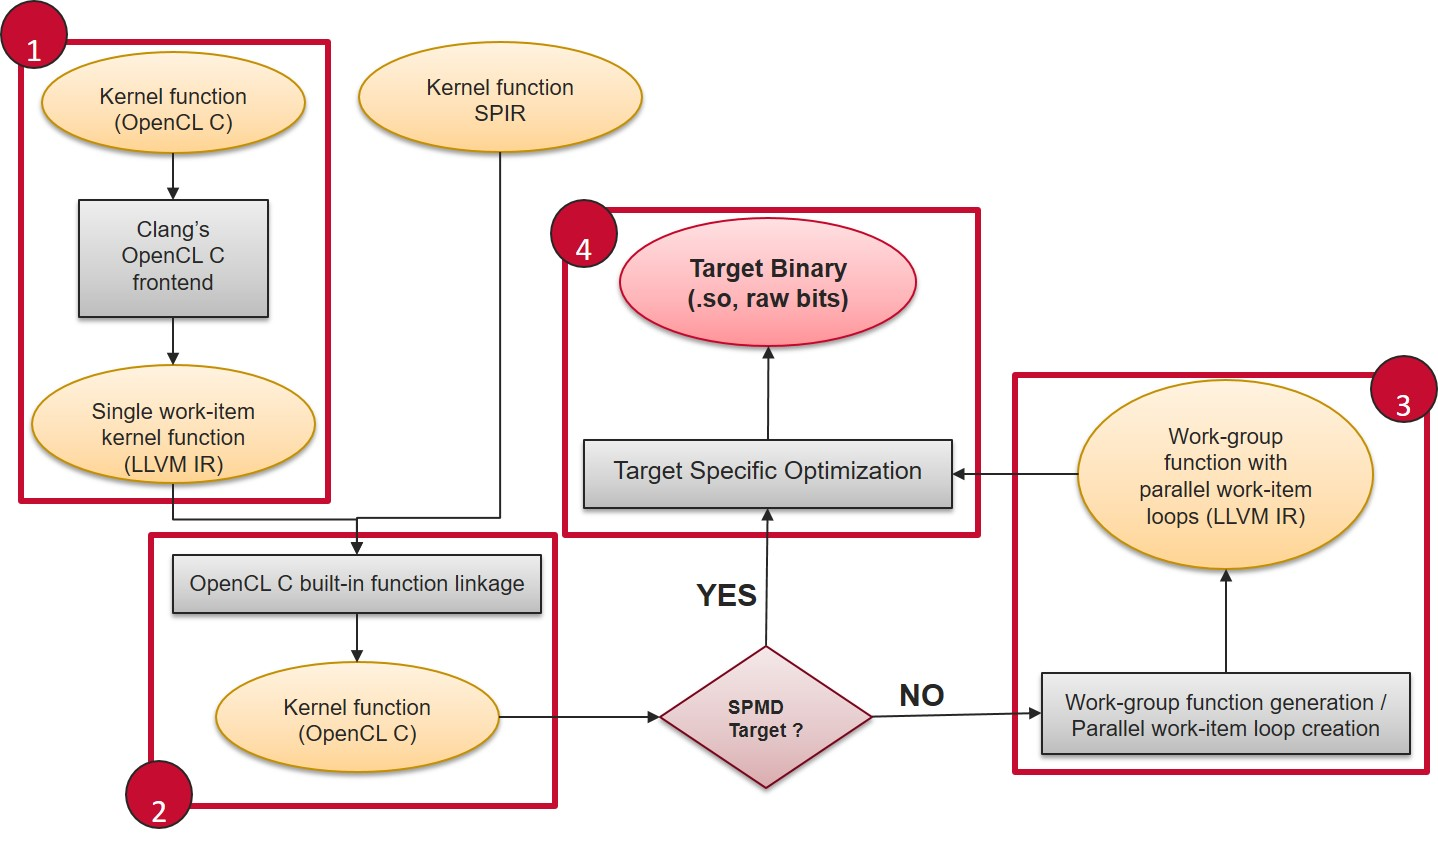
\includegraphics[width=1\textwidth]{POCL_COMPILATION_FLOW}
    \caption{POCL Kernel Compilation Flow}
    \label{fig:5_KCF}
\end{figure}

\section{Introducing new compute device to POCL}
The POCL Device layer should be included with following functionalities to add a new device. They are querying devices, managing memories, data transfers and generation of machine codes. In this context, we refer device layer as ‘basic’ device, which is a demo CPU device layer implementation. This basic device can be customized to create support for new OpenCL standard device.

\subsection{Device Query}
The host app requires the available number of devices and its device pointer for further OpenCL API calls. The Initialization function for all device types count the number of available devices using pocl\_basic\_probe() function in the device layer implementation. From user space, we can export the available device using POCL\_DEVICES with device name. When the probe function of a respective device type matches with the available environmental device name, then the devices are accounted. We can also include multiple accelerators for a device type by introducing a sysfs interface \cite{14}, which can be probed from device layer.

\subsection{Memory Management}
Using clCreateBuffer OpenCL API, read and write mode memory objects can be created for a given size. The current implementation of device layer creates memory objects in host CPU, which is  defined in pocl\_basic\_alloc\_mem\_obj(). To create memory object for an accelerator device, pocl\_basic\_alloc\_mem\_obj() should assign the memory object's mem\_ptr as a allocated memory address in the device. These memory objects are used to write and read data in device. The memory management for a new device is dependent on device's memory organization.

\subsection{Data Transfer}
The transfers are initiated by clEnqueueReadBuffer() and clEnqueueWriteBuffer() OpenCL APIs. These APIs push the read/write operations to command queue. pocl\_basic\_read() and pocl\_basic\_write() has device level definition in device layer. This can be integrated as an OpenCL Drivers with respective to device.

\subsection{Code Generation}
The conversion of kernel source code into machine code consists of the following steps.
\begin{itemize}
	\item POCL parses the kernel descriptions into LLVM IR using OpenCL C Frontend. This action is invoked inside clBuildProgram.c. The output representation is a description for single work item.
	\item Based on the targets (SPMD or not), single-work items needs to be converted to work-group function using clEnqueueNDRangeKernel().
	\item LLVM IR is converted into machine code from device layer using llvm\_codegen(). llvm\_codegen() uses the pocl's LLVM APIs to convert work group functions into native machine code. The LLVM API calls can be found in pocl\_llvm\_api.c.
	\item Allocating memory for kernel in device and writing machine code into device are defined inside pocl\_basic\_run().
\end{itemize}
To support code generation for a new device, we can reuse the OpenCL C Frontend to generate LLVM IR and the device's LLVM backend must be integrated to llvm\_codegen().

\chapter{OpenCL Driver for Zynq}
\label{ch4_OpenCL_Driver_for_Zynq}

We studied POCL software framework, which has performance portable kernel compiler. Also, we identified the necessary changes to add a new target device in POCL framework. In this chapter, we suggest a common OpenCL Driver for Zynq Platform using xillybus project. 

\section{Xillybus}
Xillybus project provides FPGA IP core design and necessary host drivers for Xilinx and Altera FPGA series. The Xillybus IP core designs are available in different licenses variants and the host drivers are open sourced for both Windows and Linux. Xillybus has an efficient DMA based solution for data transport between Linux or windows to FPGA device. It uses well known interface mechanism for both FPGA designers and host programmer developers. The design adopts interface as either of PCI Express or AXI. FPGA designers can develop the application logic that connects to the xillybus IP core through standard FIFO buffers. On the other hand, Programmer developer can use the file operations on pipes which is similar like a device file operation. They can control the data transfer using the file handler of a xillybus device file. Thus, it behaves like data streaming between FIFO buffers and the file handler opened by the application. Xillybus also provides an online tool to download the customized Xillybus IP core. We can customize parameters like expected bandwidth, number of streams etc., They estimated logic design consumption for Xilinx products are 110LUTs/Stream and 2500 LUTs with small number of RAMs  \cite{21}. Depending on host and FPGA capabilities, Xillybus can operate simultaneously up to 3.5GB/s in both directions. They also provide the source code for Linux drivers for xillybus interface. Xillybus has been used in applications like Data acquisition and playback, interfacing with required hardware, as a custom computer interface, coprocessing and more.

\section{Xillybus FPGA design interface}
Any application logic can be designed with xillybus IP. The xillybus IP core communicates data through standard FIFO buffer with the application logic. The FPGA designer has an advantage to choose the FIFO depth and the required interface with application logic. It is portable and efficient DMA based solution available both for Personal computers and Embedded Systems. The underlying communication is interfaced with either PCI Express or ARM--based AMBA bus (AXI3/AXI4). The example in the \ref{fig:1_XFI} \cite{22} gives a simplified block diagram for xillybus FPGA design interface for one data stream in each direction.
\begin{figure}[h]
    \centering
    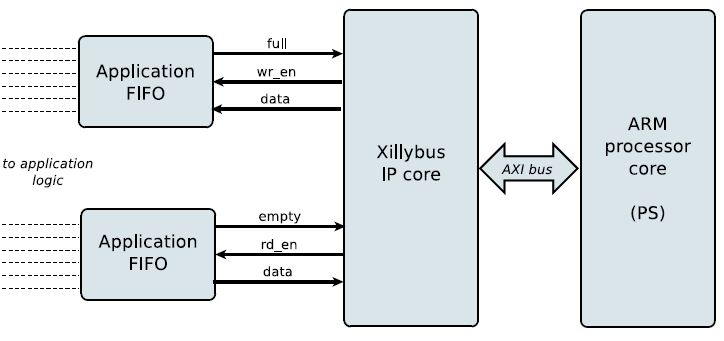
\includegraphics[width=1\textwidth]{xillybus_FPGA_Interface}
    \caption{Xillybus FPGA Interface}
    \label{fig:1_XFI}
\end{figure}

As shown in the example, when the data is written in lower FIFO buffer by application logic, the other end of the FIFO buffer senses the availability of data and transfers to the host. In the Processing System, it will be readable to the user--space software. Thus, the xillybus IP core setting relieves the FPGA designer from data traffic with the host. However, The IP manages to check the FIFOs ‘empty’ or ‘full’ signals and initiates data transfer accordingly. The xillybus is demonstrated with demo bundle which loopbacks the input and output direction FIFO buffers. These buffers in demo are configured with same clock. It cannot be used, when the FIFO are meant for cross clocking. Whenever a burst is started, xillybus IP core senses the empty or full signal and does not attempt to read from an empty buffer and to write in a full buffer. It serves all the connected buffer equally. FIFO buffers, which are getting filled fast, will be granted longer bursts. This simple arbitration gives efficient communication for the buffers that fill faster and follows low latency on FIFOs that receives little data.

\section{Xillybus Host application interface}

The Xillybus Linux host drivers generates named pipes to transfer data between FPGA and host. The Linux host drivers support any Xillybus IP configuration as it reads the required attributes from the xillybus IP core during initialization. The device file can be accessed at /dev/xillybus\_something. The device file can be opened, read and written to transfer and receive data as shown in the \ref{fig:2_HI} \cite{23}. It behaves like TCP/IP stream but on the other side it has FIFO in the FPGA. When the driver loads, FPGA is informed about the host's memory space addresses, where the DMA buffers are get allocated. The size of the buffers and number of buffers are retrieved during discovery process before allocation. Xillybus stream data can be categorized as synchronous and asynchronous based on a flag, which is fixed in FPGA’s logic. When the data flow is continuous, Asynchronous streams have better performance. During the custom IP core setting, the autoset internals can be turned off to select explicitly. The demo bundles provided, which has device files with xillybus\_write\_* and xillybus\_read\_* streams are asynchronous, while xillybus\_mem\_8 is synchronous.
\begin{figure}[h]
    \centering
    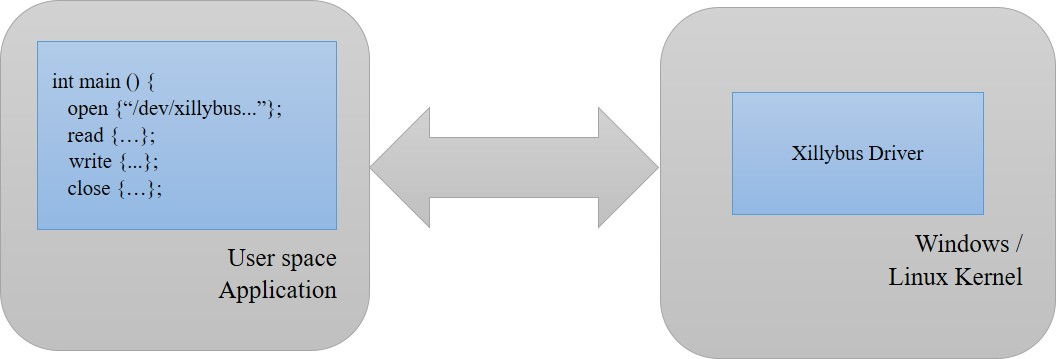
\includegraphics[width=1\textwidth]{host_interface}
    \caption{Host Interface}
    \label{fig:2_HI}
\end{figure}

For a continuous streaming process, when the hardware finished writing data to DMA buffers, it may send an interrupt to inform the software in the processing system to process the data. Similarly, the software after consuming the data, it informs the hardware to write the data again. Typically, this action is carried out using memory mapped register, where the hardware and software writes in the memory mapped register. Here, The Hardware and Software access DMA buffers in a round robin method. This technique creates the illusion of continuous data stream. Thus, the programmer can ignore the transport management when we have application data more than of DMA buffers size. 

\section{Xillybus as OpenCL Driver for Zynq Platform}
Xillybus is available for Zynq platform with customized Xillybus IP core and host Linux driver. The source code for the Linux environment are open sourced itself, but the xillybus IP core comes with variant licenses. Xillybus provides a Linux based distribution called Xillinux Distribution. It has demo drivers with host application examples. The key feature of using xillybus IP core is the design that allows the FPGA designer to connect their accelerator design or the application logic to the FIFO buffers without necessary management required for data transfer.

The motivation to develop Heterogeneous System Architecture with FPGAs is more promising in terms of power reduction, faster development and deployment. To avoid the difficulties in understanding about the underlying hardware, the parallel programming standards like OpenCL has taken over. Even though, to support a new target device for OpenCL Standard, we studied POCL software framework, which has modularized and performance portable kernel compiler for implementing OpenCL standard. POCL can be ported for Linux powered ARM--based Processing System. We propose an integration technique to use POCL framework and generalize OpenCL Implementation for Zynq Platform, which itself has a Processing System and Programmable Logic parts. To add a new device in POCL’s device layer, the first step should be the integration of OpenCL driver that can transfer the data between Processing System and the hardware device in PL. 

In POCL, ‘basic’ device layer can be customized with necessary integration for OpenCL drivers and the software package should be compiled on the platform or cross compiled to generate OpenCL Implemented library for Zynq Platform. Then using this library, host OpenCL application on Host can be build. The OpenCL drivers using xillybus host Linux drivers is targetable for any device in Programmable logic part of Zynq platform configured with xillybus IP core and application logic or accelerator design. Hence, The POCL’s basic device layer for write and read APIs can perform File operation on named pipes of xillybus IP to transfer the data between PS and PL. To increase the performance of data transfer, it is preferred to use asynchronous streaming configuration for xillybus core setting.

\section{Setting Xillinux Distribution}
The Xillinux Distribution is a development platform. This environment can be used for the custom logic in Programming Logic. Here, we discuss the steps to setup Xillinux distribution for Zedboard, which has ARM Cortex--A9 processor and a reconfigurable fabric. We must have two components to boot Xillinux distribution from a SD card. They are as follows,
\begin{itemize}\itemsep0em 
\item A FAT 32 filesystem in a boot partition that consists of bootloaders, bitstream of PL, and Linux kernel binary
\item An EXT4 root filesystem, which is mounted by Linux Operating system after loading Kernel.
\end{itemize}
We use the downloaded boot partition files, Xillinux image filesystem and the Xillybus project to boot the Zedboard with Xillinux distribution from xillybus website. 

\subsection{Unzipping the boot partition}
The xillybus project bundle for Zedboard, xillinux-eval-board-XXX.zip file is downloaded and extracted. It has following components with Verilog and VHDL files for main logic and block design files.
\begin{itemize}\itemsep0em 
\item verilog -- In src subdirectory, it contains the main logic for xillybus ip core in verilog.
\item vhdl -- In src subdirectory, the project file contains the main logic in user--editable VHDL source file.
\item cores -- Xillybus IP cores binaries are available, which are pre--compiled.
\item system -- It contains the directory for generating processor--related logic.
\item bootfiles -- This directory contains board--related binaries, which should be copied to /boot partition.
\item vivado--essentials – Contains processor--related and general--purpose logic files for use by Vivado.
\end{itemize}
The main interface file with xillybus IP core is xillydemo.v file, which is located in the ‘src’ subdirectory. These interface files can be edited to add their own data source and sinks. 

\subsection{Generating Bitstream}
Vivado design suite is a software suite developed by Xilinx for synthesis and HDL design analysis. To simplify the file structure, the bundle comes with the TCL script. The script creates a sub--directory with files as necessary. It is supported by Vivado 2014.4 or later version to run the TCL script. Following are the steps to generate bitstream for xillybus demo bundle.
\begin{enumerate}\itemsep0em 
\item Without opening new project, select Run TCL script from tools menu.
\item Browse for xillydemo--vivado.tcl script, which can be located at verilog/ subdirectory.
\item After series of events, project created message can be found in TCL console tab at Vivado’s window as shown below.
	\lstinputlisting[firstline=23, lastline=23, frame=none, basicstyle=\fontsize{11}{11}\selectfont\ttfamily, backgroundcolor=\color{gainsboro}]{code_snippet.txt}
\item After Project creation, Implementation should be run successfully. Bitstream can be created by selecting generate bitstream option on the flow navigator bar.
\item	The generated bitstream can be found at vivado/xillydemo.runs/impl\_1/
\end{enumerate}

\subsection{Loading the Linux Image}
The main task in this section is to load the system Image file to the (Micro) SD device. It can be accomplished in a Desktop environment using windows or Linux based operating system. The image file downloaded under the name xillinux.img.gz is extracted using gzip compression technique. This image contains two major partitions called boot and root. Boot partition is populated as FAT32 filesystem and it is placed with initial bootloaders and kernel binaries, while the root partition is ext4 filesystem for Linux root file system. Writing the downloaded image requires additional software and the previous content in the SD device will be deleted. We prefer to use Linux desktop environment to load the image. The following steps will write the image to SD device.
\begin{enumerate}\itemsep0em 
	\item Identifying the connected SD device name using system main log file. The log file can be found at /var/log/messages or /var/log/syslog or using dmesg linux command
	\lstinputlisting[firstline=1, lastline=8, frame=none, basicstyle=\fontsize{8}{8}\selectfont\ttfamily, backgroundcolor=\color{gainsboro}]{code_snippet.txt}
	\item The kernel will assign the name to the connected SD device, which should be like “sda” or “mmcblk”.
	\item The Downloaded image file can be uncompressed using gunzip.
	\lstinputlisting[firstline=10, lastline=10, frame=none, basicstyle=\fontsize{11}{11}\selectfont\ttfamily, backgroundcolor=\color{gainsboro}]{code_snippet.txt}
	\item We can copy the image to SD card using dd command. In the command, we should point out the correct SD device name from step 2.
	\lstinputlisting[firstline=12, lastline=12, frame=none, basicstyle=\fontsize{11}{11}\selectfont\ttfamily, backgroundcolor=\color{gainsboro}]{code_snippet.txt}
	\item After writing into SD device, we compare the content in SD device and the image file using cmp command. If we get a EOF message, the comparison is correct or If we didn’t get any message, a regular file is generated instead of writing.
	\lstinputlisting[firstline=14, lastline=15, frame=none, basicstyle=\fontsize{11}{11}\selectfont\ttfamily, backgroundcolor=\color{gainsboro}]{code_snippet.txt}
	\item The SD card device can be removed and connected back to Desktop.
	\item Copy the devicetree.dtb and boot.bin from boot partition bundle in bootfiles/ subdirectory into SD card’s boot partition. 
	\item The PL configuration bitstream, which was generated by previous section should be copied to the boot partition of SD card.
	\item Check for the following files in the boot partition.
	\begin{enumerate}\itemsep0em 
		\item uImage -- Board independent Linux Kernel file
		\item boot.bin -- The initial bootloader that has initial processor initialization and u--boot utility.
		\item devicetree.dtb -- This file is a input to the Linux kernel, which has a hardware information. It is called device tree blob.
		\item xillydemo.bit -- The Programmable Logic configuration file has an Xillybus IP core with FIFO loopback.
	\end{enumerate}
\end{enumerate}

\subsection{Booting up}
The basic peripheral connection should be a USB to UART connection between Desktop and Zedboard for debugging. The default UART setting in Zedboard is 115200 baud, 8 data bits and 1 stop bit with no flow control mechanism.  In the desktop environment, we can use Teraterm for windows or Minicom for Ubuntu Distribution with the latter UART configuration for serial port connection with Zedboard. Also, the board should be configured with the following jumper settings to change the boot source to (Micro) SD Card.
\begin{itemize}\itemsep0em 
	\item A jumper is installed in JP2 to supply 5V to USB device.
	\item JP10 and JP9 are changed from GND to 3V3 position, the other three jumpers in that row are connected to GND.
	\item A jumper is installed at JP6.
\end{itemize}

The system is powered on and booted with default environmental variables. As the root filesystem image is kept small for easy copying, it is recommended to resize the file system to the maximum. The following steps will resize the root partition with SD card’s full capacity.
\begin{enumerate}\itemsep0em 
	\item Initially, the current allocated size of the filesystem is identified using df command.
	\lstinputlisting[firstline=17, lastline=17, frame=none, basicstyle=\fontsize{11}{11}\selectfont\ttfamily, backgroundcolor=\color{gainsboro}]{code_snippet.txt}
	\item Fdisk utility is used to recreate the root filesystem. Following are the options available in fdisk.
	\begin{itemize}\itemsep0em 
	\item d [ENTER] -- Delete partition
	\item n [ENTER] -- Create a new partition
	\item w [ENTER] -- Save and quit.
	\end{itemize}
	\item By passing SD card device name to fdisk command, the second partition is deleted and a new primary partition is created with all default values. 
	\lstinputlisting[firstline=19, lastline=19, frame=none, basicstyle=\fontsize{11}{11}\selectfont\ttfamily, backgroundcolor=\color{gainsboro}]{code_snippet.txt}
	\item After rebooting the system, the filesystem can be resized using following command.
	\lstinputlisting[firstline=21, lastline=21, frame=none, basicstyle=\fontsize{11}{11}\selectfont\ttfamily, backgroundcolor=\color{gainsboro}]{code_snippet.txt}
\end{enumerate}
\chapter{Experiment and Results}
\label{ch5_Experiment_and_Results}

This chapter implements OpenCL standard for CPU and FPGA as a target device in Zynq platform. This includes POCL software framework for CPU and integration of OpenCL drivers to POCL for FPGA using xillybus. Data transfer OpenCL APIs are profiled and tested using OpenCL host application.

\section{Methodology}
The ‘basic’ device layer of POCLv0.11 is configured to use the xillybus for data transport. The customized POCL is compiled in the host system. Then the POCL library is installed with required dependencies in Xillinux Distribution on Zedboard. This library implements OpenCL for CPU and OpenCL drivers for FPGA. Programmable logic contains xillybus demo bundle IP core that loopback the input data into output FIFO buffer. The OpenCL Host application has a single kernel function which performs vector addition for ‘N’ number of inputs. The data transfer APIs for FPGA device with OpenCL standard can be tested and compared with CPU's OpenCL Implementation for different N samples of data, where each sample has 32 bit data.

The main aim of this experiment is to profile the data transfer APIs for FPGA and CPU. For, CPU we have fully implemented OpenCL ‘pthread’ device. As FPGA device in POCL has data transfer support, the kernel function is added to the hardware logic. Xillybus demo bundle can be customized with the kernel function logic. The xillydemo project is opened using TCL script in Vivado design suite. In the interface file, we introduce the kernel logic between input and output buffers. Then it is necessary to run the implementation and generate bitstream file. This process can be referred to section 4.3. The new bitstream file is copied to the boot partition of SD card and Zedboard is booted with the xillybus bitstream.
 
\section{Adding Xillybus device in POCL Framework}
The ‘basic’ device in POCL can be used for POSIX compliant device. But this device layer is customized for a new hardware. The following are the key points about the ‘basic’ device layer and changes introduced for xillybus device,
\begin{itemize}
	\item pocl\_device\_ops structure contains all the necessary function pointers for hardware related function calls. Here, we update the device name as “xillybus”. 
	\item \_cl\_device\_id structure contains hardware related information like number of compute units, device type, maximum work group size, global memory, local memory etc.,
	\item If an accelerator is attached to the xillybus, we can update the device type as CL\_DEVICE\_TYPE\_ACCELERATOR.
	\item The pocl\_basic\_probe() validates the environmental variable and the device name. If both the name matches, the hardware implementation of ‘basic’ is accounted or else pthread is used.
	\item The POCL initialization function, pocl\_basic\_init() updates the compute unit and other memory initialization.
	\item The memory allocation functions for POCL will copy the host pointer address as a new memory location inside the device layer, which is like a ‘pthread’ devices.
	\item The pocl\_basic\_read and pocl\_basic\_write are hardware data transfer APIs. By default, Basic device copies the host pointer address for both write and read operation as shown in below code snippet.
	\lstinputlisting[firstline=25, lastline=28, frame=none, numbers=left, basicstyle=\fontsize{11}{11}\selectfont\ttfamily, backgroundcolor=\color{gainsboro}]{code_snippet.txt}
	\item For FPGA device, we have xillybus host Linux device driver as an OpenCL driver. In the read and write data transfer APIs, Named pipes are used for streaming data between the Processing system and Programming Logic.
	\item We open a file pointer for /dev/xillybus\_read\_32 in Read only mode and data is read to host pointer for given size.
	\lstinputlisting[firstline=30, lastline=34, frame=none, numbers=left, basicstyle=\fontsize{11}{11}\selectfont\ttfamily, backgroundcolor=\color{gainsboro}]{code_snippet.txt}
	\item Also, we open a file pointer for /dev/xillybus\_write\_32 in Write only mode and data is written to the host pointer for given size.
	\lstinputlisting[firstline=36, lastline=40, frame=none, numbers=left, basicstyle=\fontsize{11}{11}\selectfont\ttfamily, backgroundcolor=\color{gainsboro}]{code_snippet.txt}
\end{itemize}

\section{Installing POCL}
%\subsection{Github location to install POCL}
The below url has the softwares and packages required to install POCL.

\url{https://github.com/abisheksethu/opencl-implementation}

%\subsection{Installation method}
POCL-0.11 software package can be installed on Xillinux distribution. To install pocl-0.11, we need following dependencies to be installed before POCL compilation. 
\begin{enumerate}
	\item LLVM compiler infrastructure and other LLVM sub projects like Clang and compiler-rt are required for POCL’s kernel compiler. It is available as both source code and pre-compiled binaries. LLVM-3.6 version requires host C++ toolchain version to be greater than 4.7. 
	\item Cmake package controls the compilation flow of a software using simple platform and compiler independent configuration file. We use cmake-3.7 to generate native makefiles and workspace that can be used in compiler environment. 
	\item OpenCL Installable Client Driver, ocl-icd allows multiple OpenCL Implementation for the same system that can co-exist. The OpenCL ICD loader library allows the host application to choose a platform from the installed platform and redirect the API calls to the respective platform. The POCL can be compiled with or without ICD loader. We compile using OCL ICD 2.2.10 version which is available as a source code. So, we need to compile and install the ICD loader on host System.
	\item Other dependencies like libhwloc-dev 1.8, libz-dev, libffi-dev, autoconf, libtool, ruby1.8-dev, libtinfo-dev are also installed on the host platform
	\item To profile the data transfer APIs for CPU and FPGA, we install Performance Application Programming Interface, PAPI libraries. This library 	enables the software engineer to analyze the relation between software performance with hardware in near real time.
\end{enumerate}

This work has been maintained in git hub repository under the project name opencl-implementation. It can be cloned from the above mentioned Github location. The project contains all the necessary dependency packages, poclv0.11 and the host application. The POCL’s basic layer has been customized for a new xillybus device with data transfer APIs. It also contains install script that installs all the packages and POCL. When we customize POCL software framework, POCL package can be compiled and installed separately using generated makefiles, which is available inside pocl-0.11/build sub-directory of the project.

\section{Host Application for CPU and FPGA}
The OpenCL host application performs vector addition on a given platform. This application is developed using OpenCL C APIs that can execute on a different type of device. The kernel function is written with the file extension of .cl. The kernel performs addition of two same input value and stores the output in a vector form. The host application is executed on Zedboard using POCL's OpenCL library for CPU and FPGA devices. The application code is compiled using GCC, GNU Compiler Collection with POCL’s dynamic library and PAPI’s static library. The host application executes on CPU using ‘pthread’ device layer, while it executes on FPGA using ‘xillybus’, which is a customized 'basic' device layer that has been patched for FPGA data transfer APIs. 
 
OCL-ICD 2.2.10 has been installed in Xillinux. The POCL configuration environment detects the OCL-ICD and it enables the ICD loader option for compilation. When the host OpenCL application executes, the available platforms should be available in the ICD loader file. The ICD loader file contains the path of the opencl-implementation. After installation of POCL, Path of POCL library is added to the ICD loader file which is available at /etc/OpenCL/vendors/pocl.icd location. This configuration has been included at the end of the install script.

The kernel function used in the host application is shown in code snippet. For superscalar architecture, this function can be executed by unrolling the parallel region of the kernel code such that all the work items are statically assigned to the multiple functional units. The call to get\_global\_id() returns the index of the current work item from global index space. Here the index of the work item matches with the buffer index. The main difference to C notation standard is the kernel function uses the global qualifier in the kernel arguments. 
	\lstinputlisting[firstline=42, lastline=47, frame=none, numbers=left, basicstyle=\fontsize{11}{11}\selectfont\ttfamily, backgroundcolor=\color{gainsboro}]{code_snippet.txt}

The OpenCL application flow is shown in the \ref{fig:1_HOA}. The OpenCL APIs which are responsible for platform level queries, memory allocation and data transfer are grouped into Platform APIs. The OpenCL APIs which are responsible for building the program and generating code for hardware are categorized into Runtime APIs. First, the application creates a context based on platform and device information. Second, With the context, we build and generate code for kernel function. Then the queued commands start its execution after clFinish(). The given host application is discussed in detail with a code snippet.
\begin{figure}[h]
    \centering
    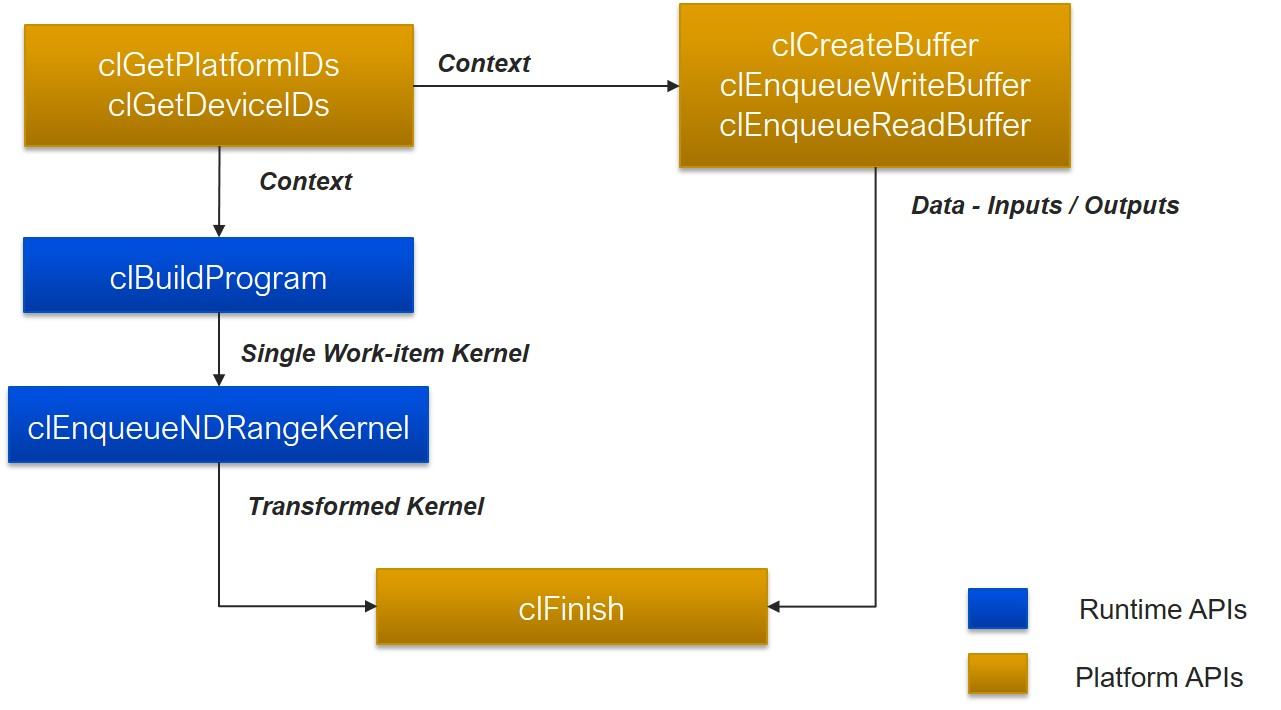
\includegraphics[width=1\textwidth]{OpenCL_APIs}
    \caption{Host Application Flow}
    \label{fig:1_HOA}
\end{figure}

\begin{itemize}
	\item The available number of platforms and its information are requested. The device ID can be obtained for a device with given device type. We have two types of device which is CPU and FPGA. This application receives device ID of any type, which is passed as a reference in the argument.
	\lstinputlisting[firstline=48, lastline=54, frame=none, numbers=left, basicstyle=\fontsize{11}{11}\selectfont\ttfamily, backgroundcolor=\color{gainsboro}]{code_snippet.txt}
	\item A context is created from the device\_id. This context has been used for entire access to the device. 
	\item There are two possible ways to load the kernel function. If we have the binary source for a kernel function, it can create the program using clCreateProgramwithBinary() function. On another hand, kernel function with .cl extension must be loaded using the source code. Then the kernel source is created using clCreateProgramwithSource(). 
	\item The key conversion of kernel function into compute kernel part is provoked by clBuildProgram() function call. Here the work item is created with LLVM Intermediate Representation. These work-item does not contain any kernel arguments or work group information. 
	\lstinputlisting[firstline=56, lastline=61, frame=none, numbers=left, basicstyle=\fontsize{11}{11}\selectfont\ttfamily, backgroundcolor=\color{gainsboro}]{code_snippet.txt}
	\item The kernel arguments for each work item is created using clSetKernelArg(). Here, the arguments are called as input and output. 
	\item A command queue is created, where the write, read and execute commands are enqueued. First Write command is enqueued using clEnqueueWriteBuffer(). The input data array is passed as one of the arguments to the function.
	\lstinputlisting[firstline=63, lastline=68, frame=none, numbers=left, basicstyle=\fontsize{11}{11}\selectfont\ttfamily, backgroundcolor=\color{gainsboro}]{code_snippet.txt}
	\item The function clEnqueueNDRangeKernel() executes the kernel over the entire range of 1D input data set. We give maximum work group size to exploit maximum parallelism for CPU. 
	\lstinputlisting[firstline=71, lastline=78, frame=none, numbers=left, basicstyle=\fontsize{11}{11}\selectfont\ttfamily, backgroundcolor=\color{gainsboro}]{code_snippet.txt}
	\item Finally, the read command is enqueued and the output data is stored in ‘results’ variable. The clFinish releases all the commands. The output data is validated from CPU and FPGA. 
\end{itemize}

The host application can be found at opencl-implementation/host\_app location in git repository. It has run script which can automate the compilation and execution environment. POCL library location is added to LD\_LIBRARY\_PATH. The execution flow is shown below.
\begin{enumerate}
	\item POCL checks for the available device in the environmental variable. This feature can be enabled by exporting the required device. First, we export ‘pthread’ device. So, the kernels are executed on CPU.
	\item Another environmental variable is updated for varied sizes of data samples. Then the host application starts its execution. This process is repeated for 1024 to 16384 samples for about 16 iterations. 
	\item Each data set is tested for 10 iterations. The timing information for all OpenCL APIs is stored in a local file.
	\item Second, we export ‘xillybus’ device to POCL\_DEVICES. Thus, the data transfers are initiated to xillybus demo bundle on FPGA and it follows step 2 and 3. As xillybus is a customized form of ‘basic’ device layer, the kernel functions are not transferred to FPGA. 
\end{enumerate}

\section{Results}
The profiling for OpenCL APIs is performed using Performance Application Programming Interface, PAPI library. The timing information is captured before and after OpenCL API calls. The kernel function and data transfers are tested with different data set samples. Each data set samples are tested for ten iterations and average time value is recorded. The timing information is measured in microseconds. For example, the current pocl device is exported as ‘pthread’ for CPU. The application is executed for 10 iterations for 1024 input vectors, where size of each input vector is 32 bit. This process is repeated up to 16384 input vectors in 16 iterations. This is also tested and profiled for the xillybus device. Though the xillybus does not receive the kernel logic from POCL, we have hard coded the hardware for same kernel logic. Thus, the data read from FPGA should match the expected output. 

\subsection{HOST to DEVICE Data Transfer}
The Data transfer between host and device are analyzed using the timing values, which are recorded in the tables \ref{tab:pthread_Table} and \ref{tab:xillybus_Table} for both pthread and xillybus devices.
% Table generated by Excel2LaTeX from sheet 'REPORT'
\begin{table}[h]
  \centering
  \begin{adjustbox}{width=0.8\textwidth}
	\small
    \begin{tabular}{|c|c|c|c|}
    \toprule
    Iteration  & Number of Samples & clEnqueueWriteBuffer & clEnqueueReadBuffer \\
    \midrule
    1     & 1024  & 84.7  & 855.3 \\
    2     & 2048  & 99.4  & 877.5 \\
    3     & 3072  & 110.8 & 884.7 \\
    4     & 4096  & 123.4 & 901.2 \\
    5     & 5120  & 143.7 & 912.4 \\
    6     & 6144  & 154.7 & 912.6 \\
    7     & 7168  & 169.5 & 920 \\
    8     & 8192  & 189.7 & 934.8 \\
    9     & 9216  & 212.1 & 949.3 \\
    10    & 10240 & 200.9 & 960.3 \\
    11    & 11264 & 217.3 & 971.2 \\
    12    & 12288 & 224.8 & 986.4 \\
    13    & 13312 & 236   & 995.5 \\
    14    & 14336 & 248.7 & 1017.6 \\
    15    & 15360 & 260   & 1041.3 \\
    16    & 16384 & 271   & 1032 \\
    \bottomrule
    \end{tabular}%
    \end{adjustbox}%
	\caption{Timing Analysis for Data Transfers APIs -- 'pthread' device}
  \label{tab:pthread_Table}%
\end{table}%
% Table generated by Excel2LaTeX from sheet 'REPORT'
\begin{table}[h]
  \centering
  \begin{adjustbox}{width=0.8\textwidth}
  \small
    \begin{tabular}{|c|c|c|c|}
    \toprule
    Iteration  & Number of Samples & clEnqueueWriteBuffer & clEnqueueReadBuffer \\
    \midrule
    1     & 1024  & 119.7 & 626.6 \\
    2     & 2048  & 123.6 & 647 \\
    3     & 3072  & 136.4 & 685.7 \\
    4     & 4096  & 140.2 & 708 \\
    5     & 5120  & 147.4 & 722.4 \\
    6     & 6144  & 154.8 & 746.7 \\
    7     & 7168  & 164.1 & 783.3 \\
    8     & 8192  & 169.4 & 803.6 \\
    9     & 9216  & 178.9 & 824.1 \\
    10    & 10240 & 186   & 846.2 \\
    11    & 11264 & 191.5 & 864.6 \\
    12    & 12288 & 201   & 886.5 \\
    13    & 13312 & 206.2 & 899.7 \\
    14    & 14336 & 217.3 & 939.9 \\
    15    & 15360 & 223   & 958.5 \\
    16    & 16384 & 235.7 & 967.8 \\
    \bottomrule
    \end{tabular}%
    \end{adjustbox}%
	\caption{Timing Analysis for Data Transfers APIs -- 'xillybus' device}
  \label{tab:xillybus_Table}%
\end{table}%


\subsection{Comparison of OpenCL APIs for pthread and xillybus device}
The Timing graph for clEnqueueWriteBuffer and clEnqueueReadBuffer OpenCL APIs are shown in figure \ref{graph1:write} and \ref{graph2:read}. We observe the xillybus device data transfers are faster than pthread device, when the number of samples are increased.
%% \hfill
%	 \begin{figure}[!b]
%	 \centering 
%	 \begin{tikzpicture}[scale = 1.1]
%	 \begin{semilogyaxis}[
%		xlabel=Datasize$(N)$,
%		ylabel=Time $(ms)$,
%	 % 	scaled ticks=base 10:-5,
%	 xtick pos=left,
%	 ytick pos=left,
%	 ymax = 600,
%	 xmax = 16777216,
%	 yticklabels={1,10,100,1000},
%	 %	symbolic y coords={0.4239,0.847,1.67,3.33,6.69,13.33,26.63,54.41,70,150,290,560},
%	 %  symbolic y coords = {-1,-0.698,-0.522,-0.397,-0.301,-0.221,-0.154,-0.0969,-0.0457,0.0,0.3010,0.4771,0.6021,0.6990,0.7782,0.8450,0.9030,0.9542,1.0,1.3010,1.4771,1.6021,1.6990,1.7782,1.8450,1.9030,1.9542,2.0,2.3010,2.4771,2.6021,2.6990,2.7782,2.8452,2.9030,2.9542,3.0},
%	 %    ytick=data, 
%	 %    yticklabels={0.1,0.2,0.3,0.4,0.5,0.6,0.7,0.8,0.9,1,2,3,4,5,6,7,8,9,10,20,30,40,50,60,70,80,90,100,200,300,400,500,600,700,800,900,1000},
%	 symbolic x coords={131072,262144,524288,1048576,2097152,4194304,8388608,16777216},
%	 enlargelimits=true,
%	 xtick=data,
%	 xticklabels={$2^{17}$,$2^{18}$,$2^{19}$,$2^{20}$,$2^{21}$,$2^{22}$,$2^{23}$,$2^{24}$},
%	 width = 10cm,
%	 xmode = normal,
%	 legend pos=north west,
%	 legend style={draw=none}
%	 ] 
	 
	 
	 % \hfill
	 \begin{figure}[!b]
	 \centering 
	 \begin{tikzpicture}[scale = 1.1]
	 \begin{semilogyaxis}[
    xlabel=Number of Samples,
	ylabel=Time $(μs)$,
	 % 	scaled ticks=base 10:-5,
	 xtick pos=left,
	 ytick pos=left,
	 ymax = 300,
	 xmax = 16384,
	 %	 ymode=log,log ticks with fixed point,
	 %	grid=major,
	   %symbolic y coords={1024, 2048, 3072, 4096, 5120, 6144, 7168, 8192, 9216, 10240, 11264, 12288, 13312, 14336, 15360, 16384},
	 %   ytick={data},
	 symbolic x coords={1024, 2048, 3072, 4096, 5120, 6144, 7168, 8192, 9216, 10240, 11264, 12288, 13312, 14336, 15360, 16384},
	 xtick=data,
	 xticklabels={1024, 2048, 3072, 4096, 5120, 6144, 7168, 8192, 9216, 10240, 11264, 12288, 13312, 14336, 15360, 16384},
	 %	symbolic y coords={0.4239,0.847,1.67,3.33,6.69,13.33,26.63,54.41,70,150,290,560},
	 width = 10cm,
	 xmode = normal,
	 legend pos=north west,
	 legend style={draw=none}
	 ]    
   
	\addplot plot coordinates {
	    (1024,     84.7)
		(2048,     99.4)
		(3072,    110.8)
		(4096,    123.4)
		(5120,    143.7)
		(6144,    154.7)
		(7168,   169.5)
		(8192,   189.7)
		(9216,     212.1)
		(10240,     200.9)
		(11264,    217.3)
		(12288,    224.8)
		(13312,    236)
		(14336,    248.7)
		(15360,   260)
		(16384,   271)
		};

	\addplot plot coordinates {
	    (1024,     119.7)
		(2048,     123.6)
		(3072,    136.4)
		(4096,    140.2)
		(5120,    147.4)
		(6144,    154.8)
		(7168,   164.1)
		(8192,   169.4)
		(9216,     178.9)
		(10240,    186)
		(11264,    191.5)
		(12288,    201)
		(13312,    206.2)
		(14336,    217.3)
		(15360,   223)
		(16384,   235.7)
		};

  

%	\legend{MXP(Byte)\\Intel i3(Byte)\\ARMv7(Byte)\\Neon(Byte)\\} 
    \legend{pthread\\xillybus\\} 
	\end{semilogyaxis}
	\end{tikzpicture} 
	\label{writebuffer} 
% \hspace{4.5cm}       $f(samples,time) = a * x ^ 2 + b* x + c$
\caption{Comparison of Write buffer API} 
\label{dag:write}

\end{figure}
\begin{figure}[h!]
	 \centering 
	 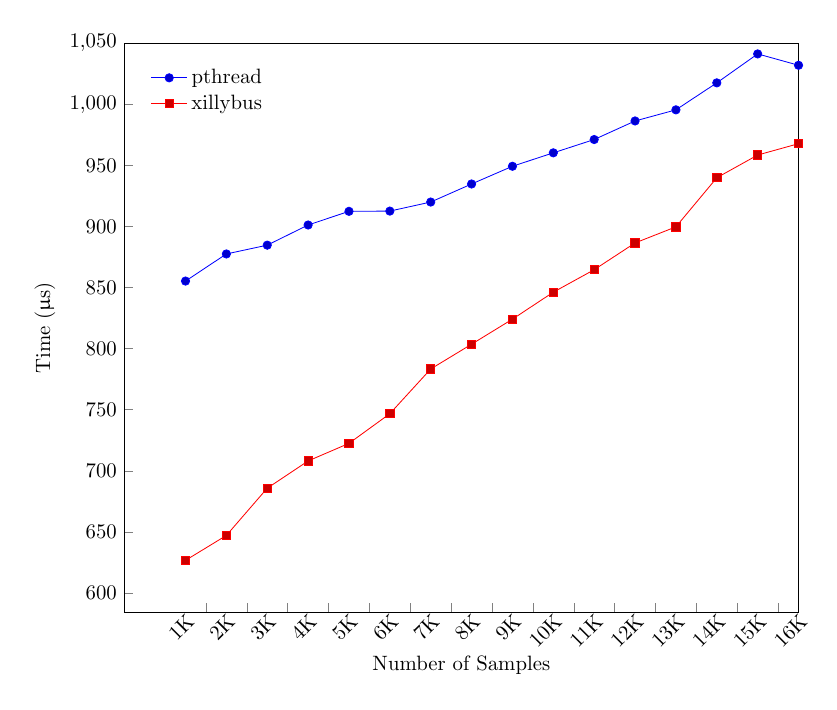
\begin{tikzpicture}[scale = 0.75]
	 \begin{axis}[
    	xlabel=Number of Samples,
		ylabel=Time ($\upmu$s),
	 	%scaled ticks=base 10:-5,
	 	xtick pos=left,
		ytick pos=left,
		ymax = 1050,
		xmax = 16384,
   		symbolic x coords={1024, 2048, 3072, 4096, 5120, 6144, 7168, 8192, 9216, 10240, 11264, 12288, 13312, 14336, 15360, 16384},
	 	xtick=data,
		xticklabels={1K, 2K, 3K, 4K, 5K, 6K, 7K, 8K, 9K, 10K, 11K, 12K, 13K, 14K, 15K, 16K},
	 	width = 13cm,
	 	xmode = normal,
	 	legend pos=north west,
	    legend style={draw=none},
	 	x tick label style={rotate=45, anchor=north east, inner sep=0mm},
		major x tick style = {opacity=0},
		minor x tick num = 1,
		minor tick length=1ex,
		every node near coord/.append style={
        anchor=west,
        rotate=90,
        font=\tiny
		},
	 ]    
   
	\addplot plot coordinates {
	    (1024,     855.3)
		(2048,     877.5)
		(3072,     884.7)
		(4096,     901.2)
		(5120,     912.4)
		(6144,     912.6)
		(7168,     920)
		(8192,     934.8)
		(9216,     949.3)
		(10240,    960.3)
		(11264,    971.2)
		(12288,    986.4)
		(13312,    995.5)
		(14336,    1017.6)
		(15360,    1041.3)
		(16384,    1032)
		};
    
	\addplot plot coordinates {
	    (1024,     626.6)
		(2048,     647)
		(3072,     685.7)
		(4096,     708)
		(5120,     722.4)
		(6144,     746.7)
		(7168,     783.3) 
		(8192,     803.6)
		(9216,     824.1)
		(10240,    846.2)
		(11264,    864.6)
		(12288,    886.5)
		(13312,    899.7)
		(14336,    939.9)
		(15360,    958.5)
		(16384,    967.8)
		};
		
    \legend{pthread\\xillybus\\} 
	\end{axis}
	\end{tikzpicture} 
	\label{writebuffer} 
	\caption{Timing Analysis for clEnqueueReadBuffer API} 
	\label{graph2:read}
\end{figure}
\chapter{Conclusions and Future Work}
\label{ch6_Conclusions_and_Future_Work}

\section{Conclusions}
The report focused on OpenCL Implementation using Portable computing language for heterogeneous system architecture. The software components of POCL supports addition of new device to implement OpenCL standard with OpenCL Drivers for data transfer and LLVM backend for OpenCL Runtime. Xillybus consists of a customizable IP core for FPGA with host Linux drivers for Zynq Platform. An accelerator can be easily attached to the xillybus IP core in a reconfigurable fabric. This report discussed on integration of POCL software for OpenCL Drivers using Xillybus host device drivers for data transfer targeted for zynq platform. It also describes the detailed installation procedure for POCL with dependencies using install script on Zedboard. The Zedboard is ported using the prebuilt binaries of Xillinux distribution.

A OpenCL host application is executed for CPU and FPGA as ‘pthread’ and ‘xillybus’ device using POCL in Zynq Platform. Data transfer APIs such as clEnqueueWriteBuffer and clEnqueueReadBuffer are profiled using PAPI Libraries. The test cases have been automated using run script. The timing behavior of the above APIs for pthread and basic devices are compared, where xillybus device responds faster than pthread device as the number of samples increases. In the above test case, CPU executes the kernel function but the kernel logic is configured in hardware. Also, the project setup is available as open source in GitHub repository. 
 

\section{Future work}
\begin{thebibliography}{1}

	\bibitem{1}H. Esmaeilzadeh, E. Blem, R. St. Amant, K. Sankaralingam, and D. Burger, \emph{Dark silicon and the end of multicore scaling}, Micro, IEEE, 32(3):122-134, May 2012.
	
	\bibitem{2}A. R. Brodtkorb, C. Dyken, T. R. Hagen, J. M. Hjelmervik, and O. O. Storaasli, \emph{State-of-the-art in heterogeneous computing.} Scientific Programming, 18(1):1-33, 2010.

	\bibitem{3}B. D. de Dinechin, D. V. Amstel, M. Poulhies, and G. Lager,\emph{Time-critical computing on a single-chip massively parallel processor.} In Proceedings of the Design, Automation and Test in Europe Conference(DATE), pages 97:197:6, 2014 
	
	\bibitem{4}B. D. de Dinechin, R. Ayrignac, P. Beaucamps, P. Couvert, B. Ganne, P. G. de Massas, F. Jacquet, S. Jones, N. M. Chaisemartin, F. Riss, \emph{A clustered manycore processor architecture for embedded and accelerated applications.} In Proceedings of the International Conference on High Performance Extreme Computing Conference (HPEC), 2013
	
	\bibitem{5}L. Gwennap, \emph{Adapteva: More ops, less watts.} Microprocessor Report, 6(13):11-02, 2011

	\bibitem{6}A. Varghese, B. Edwards, G. Mitra, and A. P. Rendell, \emph{Programming the Adapteva Epiphany 64-core network-on-chip coprocessor.} In Parallel Distributed Processing Symposium Workshops (IPDPSW), pages 984-992, May 2014
	
	\bibitem{7}A. Hodjat and I. Verbauwhede,\emph{A 21.54 gbits/s fully pipelined AES processor on FPGA.} In IEEE Symposium on FPGAs for Custom Computing Machines (FCCM), pages 308-309. IEEE, 2004.
	
	\bibitem{8}A. Descampe, F. Devaux, G. Rouvroy, B. Macq, and J. Legat,\emph{An efficient FPGA implementation of a exible JPEG2000 decoder for digital cinema}, In European Signal Processing Conference, pages 2019-2022. IEEE, 2004.
	
	\bibitem{9}O. T. Albaharna, P. Y. K. Cheung, and T. J. Clarke, \emph{On the viability of FPGA-based integrated coprocessors}, In IEEE Symposium on Field-Programmable Custom Computing Machines (FCCM), pages 206-215, 1996.
	
	\bibitem{10}S. Ahmad, V. Boppana, I. Ganusov, V. Kathail, V. Rajagopalan, and R. Wittig, \emph{A 16-nm multiprocessing system-on-chip Field-programmable gate array platform},IEEE Micro, 36(2):48-62, 2016.
	
	\bibitem{11}Xilinx Ltd. Zynq-7000 technical reference manual, \url{http://www.xilinx.com/support/documentation/user_guides/ug585-Zynq-7000-TRM.pdf}, 2013
	
	\bibitem{12}The OpenCL Specification, Version 1.2, Khronos OpenCL Working Group, Specification, Rev. 19, November 2012, \url{https://www.khronos.org/registry/cl/specs/opencl-1.2.pdf}
		
	\bibitem{13}Parker, Samuel J, \emph{An automated OpenCL FPGA compilation framework targeting a configurable, VLIW chip multiprocessor}
	
	\bibitem{14}Hugo van der Wijst, \emph{An Accelerator based on the $\uprho$-VEX Processor: An Exploration using OpenCL}
	
	\bibitem{15}Kernel De-SPMD Compilation for Texas Instruments' DSPs, \url{http://portablecl.org/texas-instruments-pocl-use-case.html}
	
	\bibitem{16}Lattner, C., Adve, V. \emph{LLVM: A compilation framework for lifelong program analysis and transformation.} In: Proceedings of International Symposium on Code Generation Optimization, p. 75 (2004)
	
	\bibitem{17}Khronos Group: SPIR 1.2 Specification for OpenCL (2014)
	
	\bibitem{18}Pekka Jaaskelainen, Carlos Sánchez de La Lama, Erik Schnetter, Kalle Raiskila, Jarmo Takala, Heikki Berg, \emph{pocl: A Performance-Portable OpenCL Implementation},International Journal of Parallel Programming, Springer. October 2015, Volume 43, Issue 5.
	
	\bibitem{19}\emph{LLVM compiler infrastructure}, \url{http://llvm.org/}
	
	\bibitem{20}\emph{Clang: A C language frontend for LLVM.}, \url{http://clang.llvm.org/}
	
	\bibitem{21}\emph{Xillybus IP core}, \url{http://xillybus.com/downloads/xillybus_product_brief.pdf}
	
	\bibitem{22}\emph{Xillybus FPGA Interface}, \url{http://xillybus.com/downloads/doc/xillybus_getting_started_zynq.pdf}
	
	\bibitem{23}\emph{Xillybus Host Interface}, \url{http://xillybus.com/downloads/doc/xillybus_getting_started_linux.pdf}	
	
\end{thebibliography}

\end{document}
